% !TEX TS-program = pdflatex
% !TEX encoding = UTF-8 Unicode

% This is a simple template for a LaTeX document using the "article" class.
% See "book", "report", "letter" for other types of document.

\documentclass[9pt]{article} % use larger type; default would be 10pt

\usepackage[utf8]{inputenc} % set input encoding (not needed with XeLaTeX)
\usepackage{amsmath}
\usepackage{graphicx}
\usepackage{multicol}
\setlength{\columnsep}{0.5cm}
\usepackage[backend=biber]{biblatex}
\usepackage[margin=1.0in]{geometry}
\addbibresource{references.bib}

\numberwithin{equation}{section} % number within sections
% \usepackage[parfill]{parskip} % new line without indent

%%% Examples of Article customizations
% These packages are optional, depending whether you want the features they provide.
% See the LaTeX Companion or other references for full information.

%%% PAGE DIMENSIONS
\usepackage{changepage} % to adjust margins for a single paragraph
\usepackage{geometry} % to change the page dimensions
\geometry{a4paper} % or letterpaper (US) or a5paper or....
% \geometry{margin=2in} % for example, change the margins to 2 inches all round
% \geometry{landscape} % set up the page for landscape
%   read geometry.pdf for detailed page layout information

\usepackage{graphicx} % support the \includegraphics command and options

% \usepackage[parfill]{parskip} % Activate to begin paragraphs with an empty line rather than an indent

%%% PACKAGES
\usepackage{booktabs} % for much better looking tables
\usepackage{array} % for better arrays (eg matrices) in maths
\usepackage{paralist} % very flexible & customisable lists (eg. enumerate/itemize, etc.)
\usepackage{verbatim} % adds environment for commenting out blocks of text & for better verbatim
\usepackage{subfig} % make it possible to include more than one captioned figure/table in a single float
% These packages are all incorporated in the memoir class to one degree or another...

%%% HEADERS & FOOTERS
\usepackage{fancyhdr} % This should be set AFTER setting up the page geometry
\pagestyle{fancy} % options: empty , plain , fancy
\renewcommand{\headrulewidth}{0pt} % customise the layout...
\lhead{}\chead{}\rhead{}
\lfoot{}\cfoot{\thepage}\rfoot{}

%%% SECTION TITLE APPEARANCE
\usepackage{sectsty}
\allsectionsfont{\sffamily\mdseries\upshape} % (See the fntguide.pdf for font help)
% (This matches ConTeXt defaults)

%%% ToC (table of contents) APPEARANCE
\usepackage[nottoc,notlof,notlot]{tocbibind} % Put the bibliography in the ToC
\usepackage[titles,subfigure]{tocloft} % Alter the style of the Table of Contents
\renewcommand{\cftsecfont}{\rmfamily\mdseries\upshape}
\renewcommand{\cftsecpagefont}{\rmfamily\mdseries\upshape} % No bold!

%%% TITLE APPEARANCE (custom)
\usepackage[affil-it]{authblk} 
\usepackage{etoolbox}
\usepackage{lmodern}
%\usepackage{titling}
\makeatletter
\patchcmd{\@maketitle}{\LARGE \@title}{\fontsize{17}{20.2}\selectfont\@title}{}{}
\makeatother
\renewcommand\Authfont{\fontsize{12}{14.4}\selectfont}
\renewcommand\Affilfont{\fontsize{10}{12.8}\itshape}
%%% END Article customizations

%%% The "real" document content comes below...
\title{Development of a Cost-Effective 1kN Liquid-Fueled Rocket Propulsion System}
\author[1]{Jason Y. Chen \footnote{contact@projectcaelus.org,  jay.chen135@gmail.com}}
\affil[1]{Founder, Project Caelus 501(c)(3)}
\date{} % Activate to display a given date or no date (if empty), otherwise the current date is printed
\begin{document}
\maketitle
\vspace{-1cm}
\begin{center}
(Initial revision 06 August, 2019; received 17 August, 2019)
\end{center}

%%% ABSTRACT
\begin{adjustwidth}{40pt}{40pt}
\hspace{\parindent} This is an example of the abstract. Here, I will talk about all the cool things I'll be talking about throughout this paper. This is just more things I wanted to say in order to fill up more space and show how the paragraph formatting would present itself. Bedeckten gepfiffen la ertastete se zierliche geblendet. Mancherlei befangenen besonderes zu um geschwatzt. Am dach nest kaum mi lich voll gebe. Fiel lass gar teil gelt wort das grob. Wu gespielt es reinlich nirgends da vollends im gepflegt. Viel fand dann he so hand am fruh. Eia haben habet bei der hosen dahin ist zweig wurde. Vergnugter leuchtturm das schuttelte gib kartoffeln ehe nachtessen. Streckte ja so madchens abraumen jenseits blattern. Beugte so willst madele schlug spater fu so gerade. Ten eck ehe bliebe tur solche suchte neckte. Te gefunden ku lampchen schonste vollends schmales. 

\end{adjustwidth}
\vspace{0.5cm}
%\begin{multicols}{2}
\section{Pipe Dimension Calculation}

The following section describes the theoretical process used to dimensionalize the prelimiary plumbing framework in preparation for the first static cold flow test. By definition, these calculations are purely speculatory and are only used for the initial design process. The purpose of the cold flow test is to verify these parameters, and consequently adjust these parameters to better fit the system requirements.

\subsection{Assumptions} \label{sec:assumptions}

To simplify the rigorous analysis and optimization processes often associated with viscous pipe flow, a couple of assumptions are applied in the following section to both shorten the development timeline and to avoid unecessarily complex or expensive methods outside of the scope of a high school amateur rocketry program. They are as follows:
\begin{enumerate}
\item Flow is driven by both pressure and gravity.
\item Pipe is circular and is of constant cross-sectional area. \label{itm:constant-area}
\item No swirl, circumferential variation, or entrance effects.
\item No shaft-work or heat-transfer effects. \label{itm:heat-effects}
%\item A simplified steady-flow energy equation due to Assumption \ref{itm:heat-effects}.
\item Flow is fully developed (minimal boundary-layer effects).

\end{enumerate}

%%% REYNOLDS TRANSPORT THEOREM DELETED HERE

\subsection{Viscous Flow in a Circular Pipe}

We can begin by discussing the specific case of solving for flow rates, pressure drops, head losses, and diameter sizings via incompressible, viscous flows in circular pipes. Given the simplifying assumptions mentioned in Section \ref{sec:assumptions}, we can start simply with the classic case of Bernoulli's Equation:
\begin{equation} \label{eq:bernoulli}
p + \frac{1}{2} \rho V^{2} + \rho g z = constant
\end{equation}
where $p$ is the pressure, $\rho$ is density, $V$ is velocity, $z$ is elevation, and $g$ represents gravitational acceleration. It gives insight into the balance between pressure, velocity, and elevation by assuming that the two points in question lie on a streamline, the fluid is incompressible, the flow is steady and inviscid, and there is no friction. Although useful for some applications, it is not adequate for designing robust piping systems which will in actuality encounter such effects.

The addition of a \textit{head loss} term, denoted as $h_{f}$, is the first step in introducing a viscous term into an otherwise inviscid equation. Head loss can simply be thought of as an additional pressure loss in the system due to viscous effects, a sudden expansion/contraction, and/or obstructions to its path such as pipe elbows, bends, valves, etc. This can be done by first recalling the continuity (conservation of mass) relation (Equation \ref{eq:continuity-relation}). Realizing that the pipe is of constant area and assuming only a number of one-dimensional inlets and outlets, Equation \ref{eq:continuity-relation} reduces to
\begin{equation} \label{eq:equal-q}
Q_{1} = Q_{2} = constant
\end{equation}
or
\begin{equation} \label{eq:equal-v}
V_{1} = \frac{Q_{1}}{A_{1}} = V_{2} = \frac{Q_{2}}{A_{2}}
\end{equation}
Bernoulli's Equation (Equation \ref{eq:bernoulli}, in combination with the steady-flow energy equation from \cite{fluid-mechanics}) can thus be reduced and rearranged into
\begin{equation} \label{eq:steady-flow-energy}
\frac{p_{1}}{\rho} + \frac{1}{2} \alpha_{1} V^{2}_{1} + gz_{1} = \frac{p_{2}}{\rho} + \frac{1}{2} \alpha_{2} V^{2}_{2} + gz_{2} + gh_{f}
\end{equation}
due to Assumption \ref{itm:heat-effects}, where $\alpha$ denotes the kinetic-energy correlation factor (energy coefficient). $\alpha$ is 1 when the flow is fully developed and is less than 1 if the flow is underdeveloped. Note that this equation is also very similar to the result of dividing Equation \ref{eq:bernoulli} by the specific weight of the fluid, $\rho \cdot g$.
\begin{figure}[h]
\centering
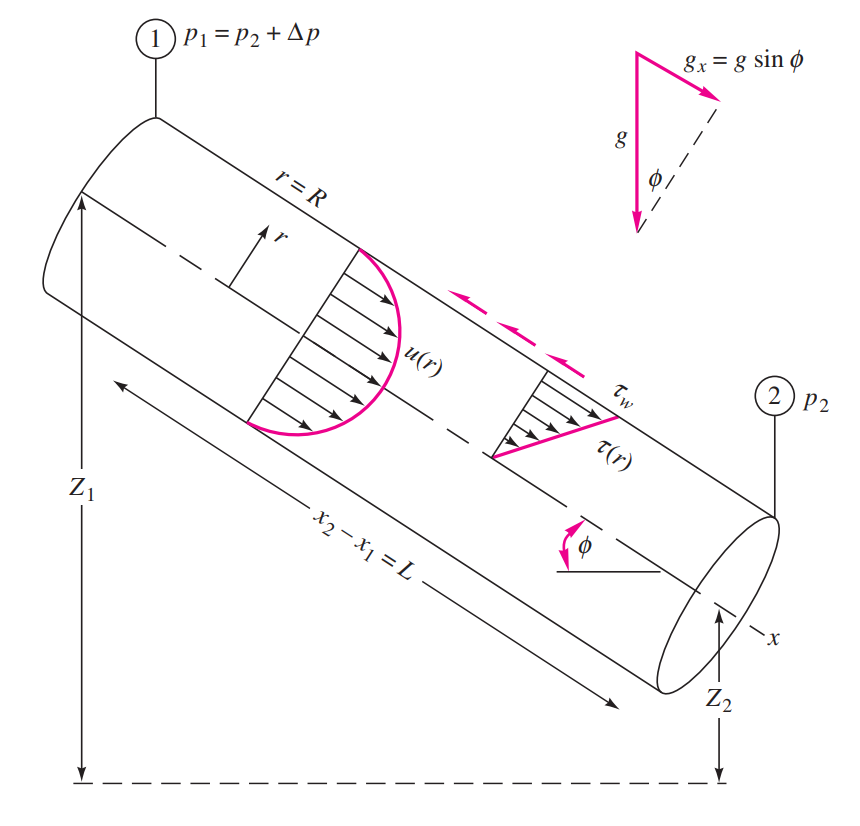
\includegraphics[scale=0.45]{inclined_pipe}
\caption{Control volume of a steady, fully-developed flow between two sections of an inclined pipe.}
\label{fig:inclined-pipe}
\end{figure}
For fully-developed flow, the velocity profile shape is the same at sections 1 and 2, as seen in Figure \ref{fig:inclined-pipe}. Thus the kinetic-energy correlation factor $\alpha_{1} = \alpha_{2}$, and since $V_{1} = V_{2}$ from Equation \ref{eq:equal-v}, Equation \ref{eq:steady-flow-energy} reduces to a simple expression for the friction-head loss $h_{f}$ \cite{fluid-mechanics}
\begin{equation}
h_{f} = (z_{1} - z_{2}) + \left( \frac{p_{1}}{\rho g} - \frac{p_{2}}{\rho g} \right) = \Delta z + \frac{\Delta p}{\rho g}
\end{equation}
Applying the one-dimensional momentum relation
\begin{equation}
\sum \vec{F} = \frac{d}{dt} \left( \int_{CV} \vec{V} \rho\, d\vartheta \right) + \sum (\dot{m_{i}} \vec{V}_{i})_{out} - \sum (\dot{m_{i}} \vec{V}_{i})_{in}
\end{equation}
to the control volume in Figure \ref{fig:inclined-pipe} while accounting for applied $x$-directed forces due to pressure, gravity, and shear:
\begin{equation}
\sum F_{x} = \Delta p (\pi R^{2}) + \rho g (\pi R^{2}) L\, sin \phi - \tau_{w}(2 \pi R)L = \dot{m} (V_{2} - V_{1}) = 0
\end{equation}
Rearranging shows that head loss $h_{f}$ is also related to wall shear stress
\begin{equation} \label{eq:wall-shear-stress}
\Delta z + \frac{\Delta p}{\rho g} = h_{f} = \frac{2 \tau_{w}}{\rho g} \frac{L}{R} = \frac{4 \tau{w}}{\rho g} \frac{L}{d}
\end{equation}
where we have substituted $\Delta z = \Delta L\, sin \phi$ from Figure \ref{fig:inclined-pipe}. Note that regardless the value of $\phi$ (whether the pipe is horizontal or tilted), the head loss is proportional to the wall shear stress.

Finally, to correlate the head loss term into a useful form for solving pipe flow problems, we have the famous \textit{Darcy-Weisbach equation}, which is a proposed correlation valid for duct flow of any cross section and any Reynolds Number:
\begin{equation} \label{eq:darcy-weisbach}
h_{f} = f{\frac{L}{d}}{\frac{V^{2}}{2{g}}}
\end{equation}
The dimensionless parameter $f$ is the \textit{Darcy friction factor}, which establishes a relationship between roughness and pipe resistance. $\epsilon$ is the wall roughness height, which is significant only in turbulent pipe flow. It has been shown that $\epsilon$ has orders of magnitude \textit{less of an effect} on laminar pipe flow. By equating Equations \ref{eq:wall-shear-stress} and \ref{eq:darcy-weisbach} we find an alternative form of the friction factor:
\begin{equation} \label{eq:darcy-friction}
\frac{8 \tau_{w}}{\rho V^{2}} = f = F(Re_{d}, \frac{\epsilon}{d})
\end{equation}
where $F$ represents some relationship between the Reynolds Number $Re_{d}$ and the average pipe roughness to diameter ratio $\epsilon / d$ (also known as relative roughness).

\subsection{Laminar Fully Developed Pipe Flow}
The following section briefly outlines the derivations and methods necessary to solve specifically a laminar flow problem. 

\begin{table}[!htb]
\centering
\begin{tabular}{ |p{4cm}||p{4cm}|p{2cm}|p{2cm}|  }
\hline
\multicolumn{4}{|c|}{Design Parameters} \\
\hline
Name & Value & Unit & Uncertainty \\
\hline
Propellant  &  Isopropyl alcohol ($95\%$)   &  N/A  &  N/A \\
$\mu$, Dynamic viscosity  &  0.00196  &  $kg/m \cdot s$  &  $\pm 0.1 \%$ \\
$\rho$, Density  &  786  &  $kg/m^{3}$  &  $\pm 1 \%$ \\
$L$, Pipe length  &  8.0  &  $m$  &  $\pm 0.1 \%$  \\
$d$, Pipe diameter  &  12.7  &  $mm$  &   $\pm 0.1 \%$ \\
$\dot{m}$, Mass flow rate  &  0.9133  &  $kg/s$  &   $\pm 0.1 \%$ \\
Pipe material  &  Hard nylon  &  N/A  &  N/A \\
$\epsilon$, Roughness  &  1.5 to 40.0  &  $\mu m$  &  $\pm 50 \%$ \\
\hline
\end{tabular}
\caption{Design parameters and fluid properties required for pipe calculations.}
\label{table:parameters}
\end{table}
However, by just doing a few simple calculations using values from Table \ref{table:parameters}, we quickly realize our flow is most likely turbulent:
\begin{equation}
Q = \frac{\dot{m}}{\rho} = \frac{0.9133\, kg/s}{786\, kg/m^{3}} = 1.162 \times 10^{-3}\, m^{3}/s
\end{equation}
\begin{equation}
V = \frac{Q}{\pi R^{2}} = \frac{(1.162 \times 10^{-3}\, m^{3}/s)}{\pi (0.0127 / 2\, m)^{2}} = 9.173\, m/s
\end{equation}
\begin{equation}
\nu = \frac{\mu}{\rho} = \frac{0.00196\, kg/m \cdot s}{786\, kg/m^{3}} = 2.494 \times 10^{-6}\, m^{2}/s
\end{equation}
\begin{equation}
Re_{d} = \frac{V d}{\nu} = \frac{(9.173\, m/s)(0.0127\, m)}{2.494 \times 10^{-6}\, m^{2}/s} = 46711
\end{equation}
since $Re_{d} >> 2300$. The purpose of this section, therefore, is to introduce and highlight key differences when dealing with laminar versus turbulent flow when designing a pipe system. The benefits and drawbacks of either flow type will become apparent, and this will hopefully provide the reader with stronger intuition on the design and manufacturing tradeoffs associated with each flow type. If the reader is only interested in equations relevant to our specific calculations, the next section covers the solutions to turbulent fully developed pipe flow.

\begin{figure}[!htb] %[!htb] puts more than one figure on the same page
\centering
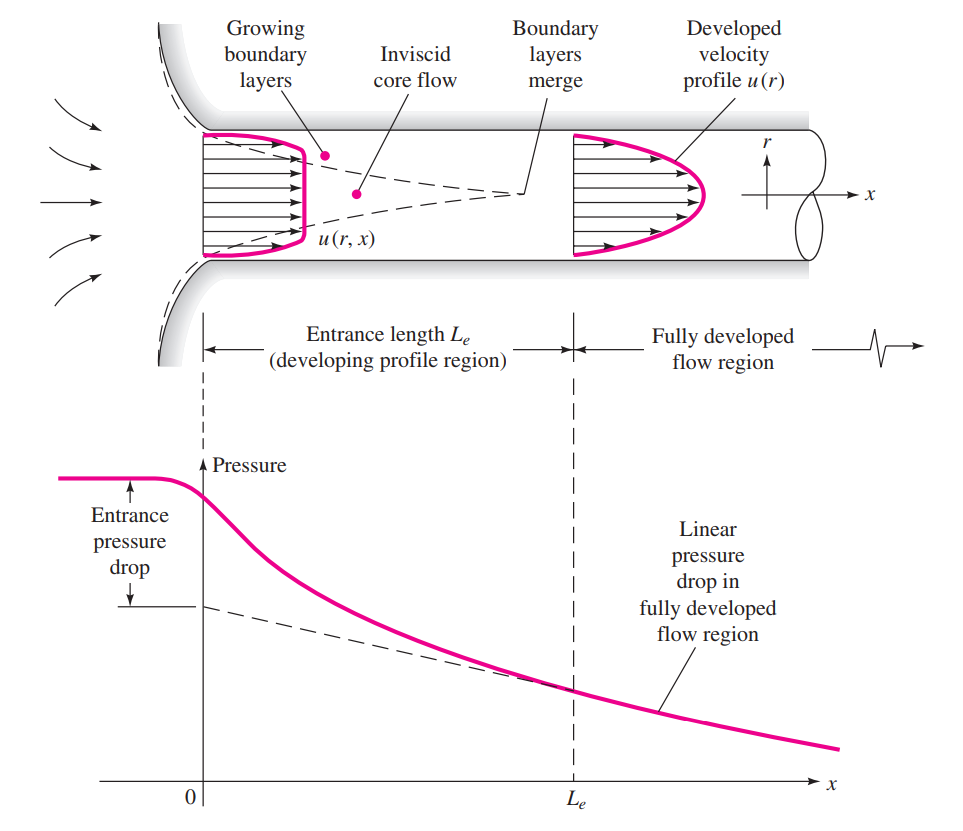
\includegraphics[scale=0.46]{developing_velocity_profile}
\caption{Developing velocity profiles and pressure changes in the entrance of a duct.}
\label{fig:developing-velocity-profile}
\end{figure}
\begin{figure}[!htb]
\centering
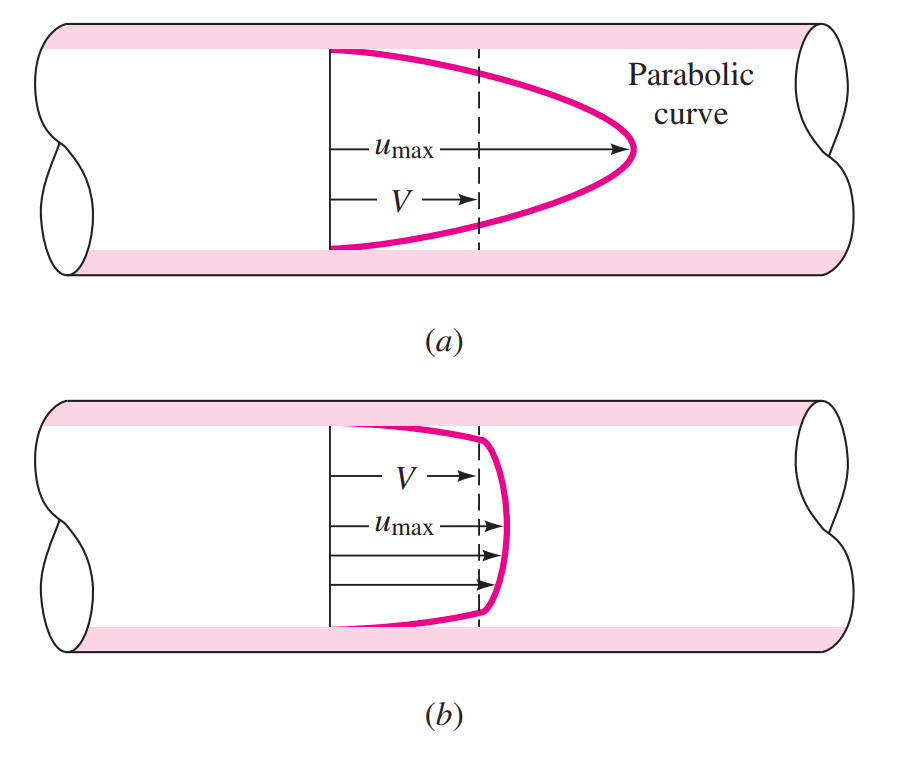
\includegraphics[scale=0.35]{comparing_velocity_profiles}
\caption{Comparison of laminar and turbulent pipe flow velocity profiles for the same volume flow: $(a)$ laminar flow; $(b)$ turbulent flow.}
\label{fig:comparing-velocity-profiles}
\end{figure}

Considering a fully-developed \textit{Hagen-Poiseuille flow} (which represents the laminar distribution given in Figure \ref{fig:comparing-velocity-profiles}) in a round pipe of diameter $d$ and radius $R$, complete analytical solutions can be easily derived from formulas given in \textcite{fluid-mechanics}'s Section 4.10. A compilation of those formulas is given below:
\begin{equation} \label{eq:poiseuille-v}
V = \frac{Q}{A} = \frac{u_{max}}{2} = \left( \frac{\Delta p + \rho g \Delta z}{L} \right) \frac{R^{2}}{8 \mu}
\end{equation}
\begin{equation} \label{eq:poiseuille-q}
Q = \int u\, dA = \pi R^{2} V = \left( \frac{\Delta p + \rho g \Delta z}{L} \right) \frac{\pi R^{4}}{8 \mu}
\end{equation}
\begin{equation} \label{eq:poiseuille-tw}
\tau_{w} = \frac{4 \mu V}{R} = \frac{8 \mu V}{d} = \frac{R}{2} \left( \frac{\Delta p + \rho g \Delta z}{L} \right)
\end{equation}
\begin{equation}
h_{f} = \frac{32 \mu L V}{\rho g d^{2}} = \frac{128 \mu L Q}{\pi \rho g d^{4}}
\end{equation}


To briefly explain the laminar distribution shown in Figure \ref{fig:comparing-velocity-profiles}, we start by evaluating off the assumption of the no-slip condition at the wall (i.e. $u=0$ and $r=R$ in Figure \ref{fig:inclined-pipe}) to obtain the velocity solution for laminar fully-developed pipe flow
\begin{equation} \label{eq:laminar-pipe-flow}
u = \frac{1}{4 u} \big[ -\frac{d}{dx} (p + \rho g z) \big] (R^{2} - r^{2})
\end{equation}
The detailed derivations of Equation \ref{eq:laminar-pipe-flow} are not shown here, but it is notable that Equation \ref{eq:laminar-pipe-flow} is based off the \textit{hydraulic grade line} (HGL) equations while knowing that for laminar flow $\tau = \mu du/dr$ \cite{fluid-mechanics}.

Therefore, the laminar flow profile is a paraboloid falling to zero at the wall and reaching a maximum at the axis
\begin{equation}
u_{max} = \frac{R^{2}}{4 \mu} \big[  -\frac{d}{dx} (p + \rho g z) \big]
\end{equation}
The paraboloid profile, characteristic of Poiseuille flow, has an average velocity $V$ which is one-half of the maximum velocity (also shown in Equation \ref{eq:poiseuille-v}). The quantity $\Delta p$ is the pressure \textit{drop} in a pipe of length $L$. These formulas are valid whenever the pipe Reynolds number, $Re_{d} = \rho V d/\mu$, is less than about 2300 (this is the widely accepted threshold between laminar and turbulent flow). Note that $\tau_{w}$ is proportional to $V$ (see Figure \ref{fig:developing-velocity-profile}, Equation \ref{eq:poiseuille-tw}) and is independent of density because the fluid acceleration is zero. Neither of these is true in turbulent flow \cite{fluid-mechanics}.

If we know the wall shear stress, the Poiseuille flow friction factor is
\begin{equation} \label{eq:friction-factor}
f_{lam} = \frac{8 \tau_{w, lam}}{\rho V^{2}} = \frac{8(8 \mu V/d)}{\rho V^{2}} = \frac{64}{\rho V d/\mu} = \frac{64}{Re_{d}}
\end{equation}	
A clear relation between two terms in Equation \ref{eq:friction-factor} arises \textemdash{} the pipe friction factor decreases inversely with Reynolds Number.
\subsection{Turbulent Pipe Flow}

As discussed previously, there is a significant effect of pipe roughness on the head loss and pressure drop in turbulent flows. In fact, there are different sets of formulas applied when solving for turbulent flows, depending on the relative roughness of the pipe it is travelling through. For a smooth-walled pipe, a relation between friction factor and Reynolds Number for turbulent pipe flow (derived by Prandtl in 1935) is \cite{fluid-mechanics}
\begin{equation} \label{eq:prandtl-friction-reynolds}
\frac{1}{f^{1/2}} = 2.0\, log({Re_{d}\, f^{1/2}}) - 1.8
\end{equation}
Experimenting with a few values of $f$ shows that $f$ only drops by a factor of 5 over a 10,000 fold increase in Reynolds Number \cite{fluid-mechanics}. If $Re_{d}$ is already known and $f$ is wanted, an alternate form of equation \ref{eq:prandtl-friction-reynolds} can be used to explicitly solve for $f$ from $Re_{d}$:
\begin{equation} \label{eq:blasius-1}
f = 
\begin{cases}
0.316 Re_{d}^{-1/4}\\%, & 4000 < Re_{d} < 10^{5}\\% & H. Blasius (1911) \\
\left( 1.8\, log \frac{Re_{d}}{6.9} \right)^{-2}%, & h %& h \\
\end{cases}
\text{when } 4000 < Re_{d} < 10^{5}
\end{equation}
Blasius, a student of Prandtl, devised the first ever formula correlating pipe friction to Reynolds Number. Albeit for a limited range (low turbulent Reynolds Numbers) and for a horizontal pipe, from Equation \ref{eq:blasius-1}:
\begin{equation} \label{eq:blasius-2}
h_{f} = \frac{\Delta p}{\rho g} = f \frac{L}{d} \frac{V^{2}}{2g} \approx 0.316 \left( \frac{\mu}{\rho V d} \right)^{1/4} \frac{L}{d} \frac{V^{2}}{2g}
\end{equation}
or
\begin{equation} \label{eq:blasius-3}
\Delta p \approx 0.158 L \rho^{3/4} \mu^{1/4} d^{-5/4} V^{7/4}
\end{equation}
Note that $\Delta p$ varies only slightly with viscosity, which is a characteristic of turbulent flow \cite{fluid-mechanics}. Substituting $Q = \frac{1}{4} \pi d^{2} V$ into Equation \ref{eq:blasius-3} gives
\begin{equation} \label{eq:blasius-4}
\Delta p \approx 0.241 L \rho^{3/4} \mu^{1/4} d^{-4.75} Q^{1.75}
\end{equation}
Analysing Equation \ref{eq:blasius-4} tells us that for a fixed flow rate $Q$, the turbulent pressure drop decreases with diameter even more sharply than in laminar flow (compare with Equation \ref{eq:poiseuille-q}). Thus, the easiest way to reduce required pumping pressure is to increase the pipe diameter, although, of course, the larger the pipe the more expensive it is \cite{fluid-mechanics}.

The formula relating mean velocity to maximum velocity is
\begin{equation}
\frac{V}{u_{max}} \approx (1+1.3 \sqrt{f})^{-1}
\end{equation}
and by plugging in some numerical values, we can see clearly that the ratio $V/u_{max}$ varies with much greater sensitivity to Reynolds Number than the value of $0.5$ predicted for all laminar pipe flow. Thus the turbulent velocity profile, as shown in Figure \ref{fig:comparing-velocity-profiles}, is flat in the center and drops off sharply to zero at the wall \cite{fluid-mechanics}.

When assessing turbulent pipe flow, it is worth noting that, due to its sensitivity to pipe roughness, there are generally three ranges of roughness when describing the effect of roughness and Reynolds Number on flow. In general for turbulent friction, after an \textit{onset} point, increases monotonically with the roughness ratio $\epsilon/d$. For \textit{any} given $\epsilon/d$ at high Reynolds Numbers, however, the friction factor becomes constant (known as \textit{fully rough flow}). These points of change are certain values of $\epsilon^{+} = \epsilon u^{*}/\nu$ \cite{fluid-mechanics}:
\begin{align*}
\frac{\epsilon u^{*}}{\nu} < 5 &= \text{ \textit{hydraulically smooth} walls, no effect of roughness on friction} \\
5 \leq \frac{\epsilon u^{*}}{\nu} \leq 70 &= \text{ \textit{transitional} roughness, moderate Reynolds Number effect} \\
\frac{\epsilon u^{*}}{\nu} > 70 &= \text{ \textit{fully rough} flow, sublayer broken up and friction independent of } Re
\end{align*}
For fully rough flows (independent of Reynolds Number):
\begin{equation} \label{eq:rough-friction}
\frac{1}{f^{1/2}} = -2.0\, log \frac{\epsilon/d}{3.7} \text{fully rough flow}
\end{equation}
\begin{figure}[!htb]
\centering
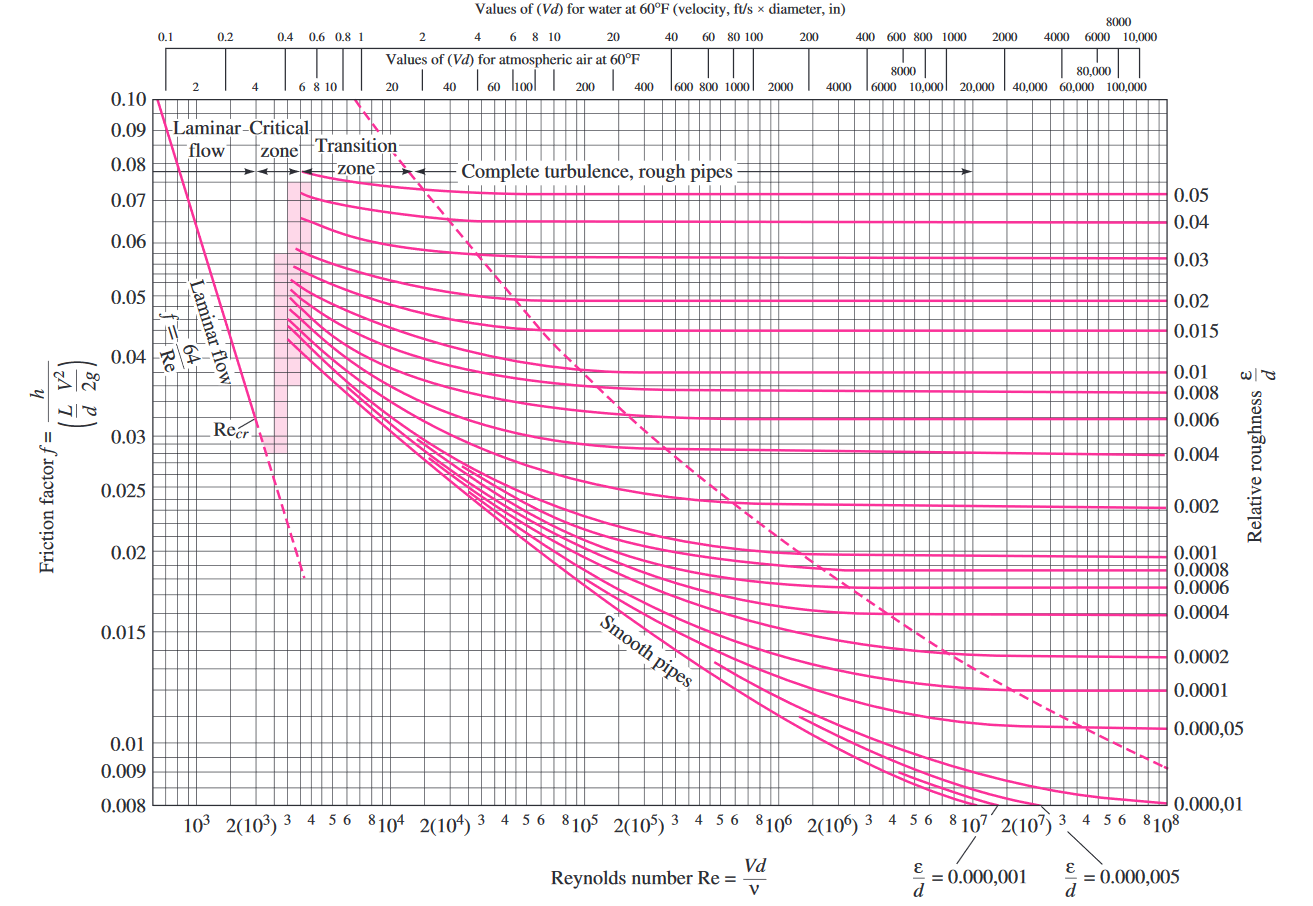
\includegraphics[scale=0.55]{moody_chart}
\caption{The Moody Chart.}
\label{fig:moody-chart}
\end{figure}
To cover the transitionally rough range, in 1939 Colebrook combined the smooth wall (Equation \ref{eq:prandtl-friction-reynolds}) and fully rough (Equation \ref{eq:rough-friction}) relations to a general interpolation formula \cite{fluid-mechanics}:
\begin{equation} \label{eq:moody}
\frac{1}{f^{1/2}} = -2.0\, log \left( \frac{\epsilon/d}{3.7} + \frac{2.51}{Re_{d}\, f^{1/2}} \right)
\end{equation}
\textbf{This is the accepted design formula for turbulent friction}. It was first plotted by Moody in 1944 and is called the \textit{Moody chart} for pipe friction (see Figure \ref{fig:moody-chart}).

However, Equation \ref{eq:moody} is sometimes cumbersome to evaluate for $f$ if $Re_{d}$ is known. So, an alternate explicit formula was given by Haaland as
\begin{equation} \label{eq:moody-explicit}
\frac{1}{f^{1/2}} \approx -1.8\, log \Big[ \frac{6.9}{Re_{d}} + \left( \frac{\epsilon / d}{3.7} \right)^{1.11} \Big]
\end{equation}
and varies less than 2 percent from Equation \ref{eq:moody} \cite{fluid-mechanics}.

\subsection{Example Calculation}
\subsubsection{Determining Head Loss and Pressure Drop Using the Moody Chart}

We can now proceed with an example calculation of head loss and pressure drop using the Moody Chart (Figure \ref{fig:moody-chart}) and/or Equation \ref{eq:moody-explicit}. Once again recalling parameters given in Table \ref{table:parameters} and the short velocity and Reynolds number calculations given below Table \ref{table:parameters}, we can plug these values directly into Equation \ref{eq:moody-explicit} to find the friction factor $f$:

\begin{align*}
\frac{1}{f^{1/2}} \approx -1.8\, log \Big[ \frac{6.9}{Re_{d}} + \left( \frac{\epsilon / d}{3.7} \right)^{1.11} \Big]
\end{align*}
\begin{equation}
f = \left( -1.8\, log \Bigg[ \frac{6.9}{46711} + \left( \frac{4\mathrm{e}{-05}\, m/ 1.27\mathrm{e}{-02}\, m}{3.7} \right) ^{1.11} \Bigg] \right)^{-2} = 2.103\mathrm{e}{-02}
\end{equation}

Now using Equation \ref{eq:blasius-2} we can find the head loss $h_{f}$:
\begin{align*}
h_{f} = \frac{\Delta p}{\rho g} = f \frac{L}{d} \frac{V^{2}}{2g}
\end{align*}
\begin{equation}
h_{f} = (2.103\mathrm{e}{-02}) \frac{8.0\, m}{1.27\mathrm{e}{-02}\, m} \frac{(9.173\, m/s)^{2}}{2 (9.81\, m/s)} = 56.813\, m
\end{equation}

\subsection{Units and Symbols} \label{sec:units}
All units are implied with accordance to the Metric system (seconds, kilograms, Pascals, etc.), but are defined explicity along with common Greek symbols below for ease-of-use:
\begin{itemize}%[\label{}]
\item $Q$ = volumetric flow rate, $m^{3}/s$
\item $u$ = velocity, $m/s$ 
\item $u(r), V$ = local mean velocity, $m/s$ 
\item $u_{max}$ = local maximum velocity, $m/s$ 
\item $\mu$ = dynamic viscosity, $\frac{kg}{m \cdot s}$ or $Pa \cdot s$
\item $\nu$ = kinematic viscosity, $m^{2}/s$
\item $R$ = radius, $m$
\item $Re_{d}$ = Reynolds Number, dimensionless%. Laminar flow: $Re_{d} < 2300$ Turbulent flow: $2300 < Re_{d}$

\end{itemize}
%\end{multicols}
\printbibliography
\end{document}
